% REMEMBER: You must not plagiarise anything in your report. Be extremely careful.

\documentclass{l4proj}

    
%
% put any additional packages here
%

\begin{document}

%==============================================================================
%% METADATA
\title{Augmented Reality Flatpack Furniture Assembly}
\author{Paul Doherty}
\date{March 22, 2024}

\maketitle

%==============================================================================
%% ABSTRACT
\begin{abstract}
    Every abstract follows a similar pattern. Motivate; set aims; describe work; explain results.
    \vskip 0.5em
    ``XYZ is bad. This project investigated ABC to determine if it was better. 
    ABC used XXX and YYY to implement ZZZ. This is particularly interesting as XXX and YYY have
    never been used together. It was found that  
    ABC was 20\% better than XYZ, though it caused rabies in half of subjects.''
\end{abstract}

%==============================================================================

% EDUCATION REUSE CONSENT FORM
% If you consent to your project being shown to future students for educational purposes
% then insert your name and the date below to  sign the education use form that appears in the front of the document. 
% You must explicitly give consent if you wish to do so.
% If you sign, your project may be included in the Hall of Fame if it scores particularly highly.
%
% Please note that you are under no obligation to sign 
% this declaration, but doing so would help future students.
%
%\def\consentname {My Name} % your full name
%\def\consentdate {20 March 2018} % the date you agree
%

\def\consentname {Paul Kieran Doherty} % your full name
\def\consentdate {13 February 2024} % the date you agree

\educationalconsent

%==============================================================================
\tableofcontents

%==============================================================================
%% Notes on formatting
%==============================================================================
% The first page, abstract and table of contents are numbered using Roman numerals and are not
% included in the page count. 
%
% From now on pages are numbered
% using Arabic numerals. Therefore, immediately after the first call to \chapter we need the call
% \pagenumbering{arabic} and this should be called once only in the document. 
%
% Do not alter the bibliography style.
%
% The first Chapter should then be on page 1. You are allowed 40 pages for a 40 credit project and 30 pages for a 
% 20 credit report. This includes everything numbered in Arabic numerals (excluding front matter) up
% to but excluding the appendices and bibliography.
%
% You must not alter text size (it is currently 10pt) or alter margins or spacing.
%
%
%==================================================================================================================================
%
% IMPORTANT
% The chapter headings here are **suggestions**. You don't have to follow this model if
% it doesn't fit your project. Every project should have an introduction and conclusion,
% however. 
%
%==================================================================================================================================
\chapter{Introduction}

% reset page numbering. Don't remove this!
\pagenumbering{arabic} 

Augmented Reality (AR) devices are becoming increasingly commonplace in today's market with the ever improving tracking technology. As more devices become available, AR technology becomes more accessible to the average person. 

Why should the reader care about what are you doing and what are you actually doing?
\section{Guidance}

\textbf{Motivate} first, then state the general problem clearly. 

\section{Writing guidance}
\subsection{Who is the reader?}

This is the key question for any writing. Your reader:

\begin{itemize}
    \item
    is a trained computer scientist: \emph{don't explain basics}.
    \item
    has limited time: \emph{keep on topic}.
    \item
    has no idea why anyone would want to do this: \emph{motivate clearly}
    \item
    might not know \emph{anything} about your project in particular:
    \emph{explain your project}.
    \item
    but might know precise details and check them: \emph{be precise and
    strive for accuracy.}
    \item
    doesn't know or care about you: \emph{personal discussions are
    irrelevant}.
\end{itemize}

Remember, you will be marked by your supervisor and one or more members
of staff. You might also have your project read by a prize-awarding
committee or possibly a future employer. Bear that in mind.

\subsection{References and style guides}
There are many style guides on good English writing. You don't need to
read these, but they will improve how you write.

\begin{itemize}
    \item
    \emph{How to write a great research paper} \cite{Pey17} (\textbf{recommended}, even though you aren't writing a research paper)
    \item
    \emph{How to Write with Style} \cite{Von80}. Short and easy to read. Available online.
    \item
    \emph{Style: The Basics of Clarity and Grace} \cite{Wil09} A very popular modern English style guide.
    \item
    \emph{Politics and the English Language} \cite{Orw68}  A famous essay on effective, clear writing in English.
    \item
    \emph{The Elements of Style} \cite{StrWhi07} Outdated, and American, but a classic.
    \item
    \emph{The Sense of Style} \cite{Pin15} Excellent, though quite in-depth.
\end{itemize}

\subsubsection{Citation styles}

\begin{itemize}
\item If you are referring to a reference as a noun, then cite it as: ``\citet{Orw68} discusses the role of language in political thought.''
\item If you are referring implicitly to references, use: ``There are many good books on writing \citep{Orw68, Wil09, Pin15}.''
\end{itemize}

There is a complete guide on good citation practice by Peter Coxhead available here: \url{http://www.cs.bham.ac.uk/~pxc/refs/index.html}. 
If you are unsure about how to cite online sources, please see this guide: \url{https://student.unsw.edu.au/how-do-i-cite-electronic-sources}.

\subsection{Plagiarism warning}

\begin{highlight_title}{WARNING}
    
    If you include material from other sources without full and correct attribution, you are commiting plagiarism. The penalties for plagiarism are severe.
    Quote any included text and cite it correctly. Cite all images, figures, etc. clearly in the caption of the figure.
\end{highlight_title}


%==================================================================================================================================
\chapter{Background}
What did other people do, and how is it relevant to what you want to do?
\section{Guidance}
\begin{itemize}    
    \item
      Don't give a laundry list of references.
    \item
      Tie everything you say to your problem.
    \item
      Present an argument.
    \item Think critically; weigh up the contribution of the background and put it in context.    
    \item
      \textbf{Don't write a tutorial}; provide background and cite
      references for further information.
\end{itemize}

%==================================================================================================================================
\chapter{Analysis/Requirements}

\section{Analysis of Problem}

An AR solution to flatpack furniture instructions is required in the problem. These instructions are commonly paper-based and give a picture-by-picture guide to assembling the furniture, as shown in figure \ref{fig:instructions}. Taking this to the world of augmented reality opens up a plethora of opportunities. AR takes digital content into the real 3D world and is much more dynamic and fluid than the 2D paper methods.

Creating a new AR platform to communicate instructions on assembling flatpack furniture to a user requires the translation of certain concepts into an AR environment. For this to be done effectively, a user must be able to fully follow through with the instructions without any outside help or guessing. To ensure that this is the case, a set of requirements have been created for the platform to follow.

\section{Functional Requirements}

\subsection{Requirements from Paper Instructions}

It was important to analyse the paper instructions provided with a set of flatpack furniture to understand the baseline that the AR instructions would be compared to. The paper instructions for the IKEA HEMNES bedside table \ref{fig:instructions} were inspected to find the most important factors in helping a person assemble furniture.

\begin{figure}[hbt!]
    \centering
    \includegraphics[width=1\linewidth]{dissertation//images/instructions.jpg}
    \caption{Paper instructions for IKEA HEMNES bedside table}
    \label{fig:instructions}
\end{figure}

There are a few important techniques used in these instructions that can be carried over as requirements for the AR instructions. These features are key to making it clear to a user how to progress in assembly. The requirements gained from assessment of the paper instructions include:

\begin{itemize}
    \item Making it clear where a part goes
    \item Showing the direction a part should be added in
    \item Showing the orientation a part should be added in
    \item Communicating if a component needs to be assembled separately then added to the full assembly after
    \item Declaring when a part should be screwed in
    \item Giving a position to place the work in progress assembly when adding a new part
    \item Showing a close up view of smaller parts
    \item Always having access to a view of the finished product
\end{itemize}

\subsection{Requirements of Augmented Reality}

\subsection{Hardware Limitations}



\section{Non-Functional Requirements}


%==================================================================================================================================
\chapter{Design}

\section{Object Tracking}

The biggest feature of the application is showing the user how to add a part to the assembly. It was important that this was designed in a way that took advantage of the AR environment. The first chosen method to demonstrate a step was to track the parts in real life using the camera and a 3D model tracker. When an object is detected in the view, an overlay of the 3D model in red is displayed in the same position. The same model is also displayed in the position it should be placed in a blue colour. When the real part is tracked to be in the same position and rotation as is required then it is turned greed to show that it is correct.

\section{Animation Visualisation}

\section{Instructions System Architecture}

One of the most important goals of the project was translating a set of paper instructions to a digital, 3D format. A system was required that broke a piece of furniture up into each of its parts which would then be added in a particular step. The system would contain all of the required information about each part and step which could then be taken and visualised in the engine used.

\begin{figure}[hbt!]
    \centering
    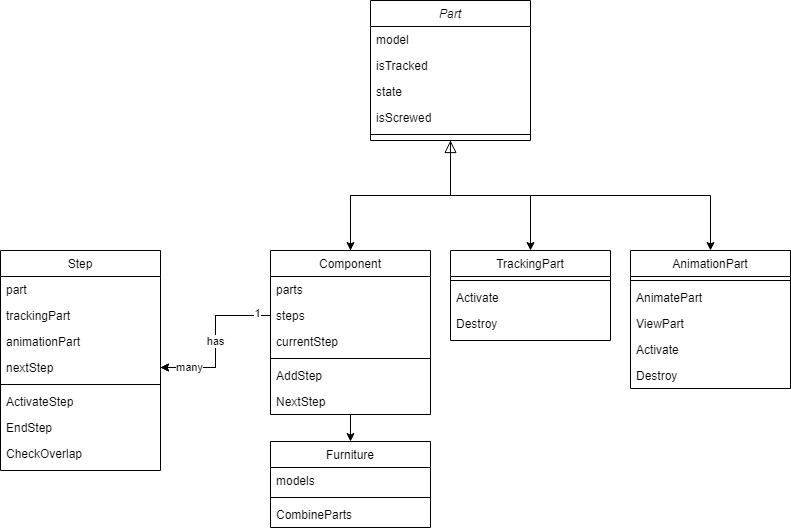
\includegraphics[width=0.8\linewidth]{dissertation//images/classDiagram.jpg}
    \caption{Class diagram showing the set up of the instructions system}
    \label{fig:classDiagram}
\end{figure}

% Maybe add parent position and rotation to Part ^^^

The system is designed to step through parts in the order of the instructions. \textit{Furniture} is the base object that will be created in the engine. As a child of \textit{Component} it has a list of parts which can either be a \textit{Part} or \textit{Component}. It is provided with models which are set up in a particular way, as shown in chapter \ref{modelSetup}, which allows it to convert each model to a \textit{Part} or \textit{Component} and put them in the correct order into the parts list. If a model is standalone with no children, meaning it should just be added to the assembly by itself, it is a \textit{Part}. If the model has children, meaning it should be assembled separately then added to the full assembly, it is a \textit{Component}. For each item in this list there is also a \textit{Step} or list of steps. Each \textit{Component} has a list of steps and a current step. A \textit{Step} has a \textit{Part}, \textit{TrackingPart}, \textit{AnimationPart}, and a \textit{Step} which points to the next \textit{Step} in the order of the instructions. The AddStep function adds a \textit{Step} to the list based on a given \textit{Part}/\textit{Component} and automatically determines which type it is. For a \textit{Part} it will simply add a new \textit{Step} and set it as the nextStep of the previous one. For a \textit{Component} it will set the nextStep of the previous \textit{Step} to the first \textit{Step} of the \textit{Component} and the final item of its steps will point to a new \textit{Step} created for the \textit{Component} itself. A \textit{Part} has a model which would exist in the world space. It can either be tracked or animated and it can be screwed in. It has a state which can be either disabled, waiting, correct or finished. These represent the progress through a step of the instructions. If a \textit{Part} is tracked then its corresponding \textit{Step} will use a \textit{TrackingPart}, otherwise it will use an \textit{AnimationPart}. A \textit{TrackingPart} will automatically be connected to the object tracking system when created and will track its real life counterpart. An \textit{AnimationPart} automatically starts animating the motion of adding the part when created. The ActivateStep and EndStep methods of \textit{Step} will choose the right type of part to create and destroy when the step is active.

\section{Model Setup} \label{modelSetup}

In order to visualise the system there had to be 3D models for each part of the assembly. Each model had to be accurate and positioned correctly relative to the other models. In order to accomplish this a template was designed which would automatically integrate with the instructions system. 

\begin{figure}[hbt!]
    \centering
    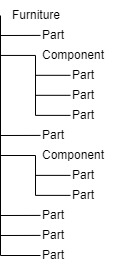
\includegraphics[width=0.2\linewidth]{dissertation//images/modelFileStructure .jpg}
    \caption{Example model structure to be provided to the instructions system}
    \label{fig:modelStruct}
\end{figure}

Each part is an individual 3D model which can be grouped together to make a component or left alone. All components and parts are then grouped to the full furniture model and positioned correctly. Once this model is correct, a list of each part and component is created which is ordered in the order of when parts are added. The list also contains a position and rotation which the parent of a part should moved to while the part is being added.

How is this problem to be approached, without reference to specific implementation details? 
\section{Guidance}
Design should cover the abstract design in such a way that someone else might be able to do what you did, but with a different language or library or tool.

%==================================================================================================================================
\chapter{Implementation}

\section{Choosing Platforms}

\section{Unity}

\section{Tracking Method}

\subsection{Unity Image Tacking}

\subsection{Azure Object Anchors}

\subsection{VisionLib}

\section{Licensing Troubles}

\section{Setting Up Project}
% ^ These could be combined v
\section{Scene Set Up}

\section{Custom Framework for Instructions}

\section{Input}

\section{Custom 3D Models}
% Positions set relative to parent
\section{Setup of Bedside Table Prefab}

What did you do to implement this idea, and what technical achievements did you make?
\section{Guidance}
You can't talk about everything. Cover the high level first, then cover important, relevant or impressive details.



\section{General points}

These points apply to the whole dissertation, not just this chapter.



\subsection{Figures}
\emph{Always} refer to figures included, like Figure \ref{fig:relu}, in the body of the text. Include full, explanatory captions and make sure the figures look good on the page.
You may include multiple figures in one float, as in Figure \ref{fig:synthetic}, using \texttt{subcaption}, which is enabled in the template.



% Figures are important. Use them well.
\begin{figure}
    \centering
    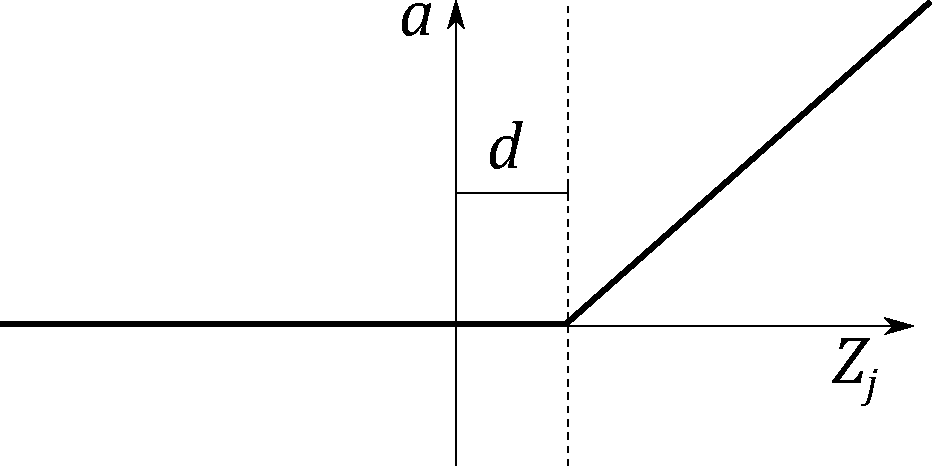
\includegraphics[width=0.5\linewidth]{images/relu.pdf}    

    \caption{In figure captions, explain what the reader is looking at: ``A schematic of the rectifying linear unit, where $a$ is the output amplitude,
    $d$ is a configurable dead-zone, and $Z_j$ is the input signal'', as well as why the reader is looking at this: 
    ``It is notable that there is no activation \emph{at all} below 0, which explains our initial results.'' 
    \textbf{Use vector image formats (.pdf) where possible}. Size figures appropriately, and do not make them over-large or too small to read.
    }

    % use the notation fig:name to cross reference a figure
    \label{fig:relu} 
\end{figure}


\begin{figure}
    \centering
    \begin{subfigure}[b]{0.45\textwidth}
        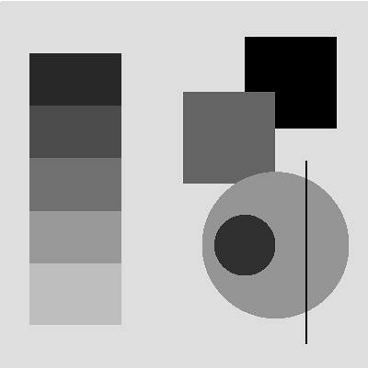
\includegraphics[width=\textwidth]{images/synthetic.png}
        \caption{Synthetic image, black on white.}
        \label{fig:syn1}
    \end{subfigure}
    ~ %add desired spacing between images, e. g. ~, \quad, \qquad, \hfill etc. 
      %(or a blank line to force the subfigure onto a new line)
    \begin{subfigure}[b]{0.45\textwidth}
        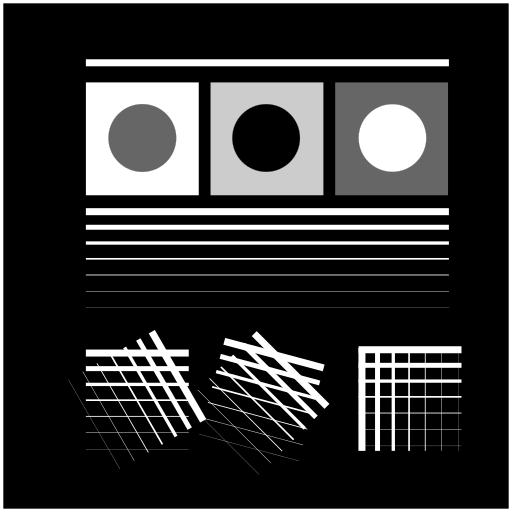
\includegraphics[width=\textwidth]{images/synthetic_2.png}
        \caption{Synthetic image, white on black.}
        \label{fig:syn2}
    \end{subfigure}
    ~ %add desired spacing between images, e. g. ~, \quad, \qquad, \hfill etc. 
    %(or a blank line to force the subfigure onto a new line)    
    \caption{Synthetic test images for edge detection algorithms. \subref{fig:syn1} shows various gray levels that require an adaptive algorithm. \subref{fig:syn2}
    shows more challenging edge detection tests that have crossing lines. Fusing these into full segments typically requires algorithms like the Hough transform.
    This is an example of using subfigures, with \texttt{subref}s in the caption.
    }\label{fig:synthetic}
\end{figure}

\clearpage

\subsection{Equations}

Equations should be typeset correctly and precisely. Make sure you get parenthesis sizing correct, and punctuate equations correctly 
(the comma is important and goes \textit{inside} the equation block). Explain any symbols used clearly if not defined earlier. 

For example, we might define:
\begin{equation}
    \hat{f}(\xi) = \frac{1}{2}\left[ \int_{-\infty}^{\infty} f(x) e^{2\pi i x \xi} \right],
\end{equation}    
where $\hat{f}(\xi)$ is the Fourier transform of the time domain signal $f(x)$.

\subsection{Algorithms}
Algorithms can be set using \texttt{algorithm2e}, as in Algorithm \ref{alg:metropolis}.

% NOTE: line ends are denoted by \; in algorithm2e
\begin{algorithm}
    \DontPrintSemicolon
    \KwData{$f_X(x)$, a probability density function returing the density at $x$.\; $\sigma$ a standard deviation specifying the spread of the proposal distribution.\;
    $x_0$, an initial starting condition.}
    \KwResult{$s=[x_1, x_2, \dots, x_n]$, $n$ samples approximately drawn from a distribution with PDF $f_X(x)$.}
    \Begin{
        $s \longleftarrow []$\;
        $p \longleftarrow f_X(x)$\;
        $i \longleftarrow 0$\;
        \While{$i < n$}
        {
            $x^\prime \longleftarrow \mathcal{N}(x, \sigma^2)$\;
            $p^\prime \longleftarrow f_X(x^\prime)$\;
            $a \longleftarrow \frac{p^\prime}{p}$\;
            $r \longleftarrow U(0,1)$\;
            \If{$r<a$}
            {
                $x \longleftarrow x^\prime$\;
                $p \longleftarrow f_X(x)$\;
                $i \longleftarrow i+1$\;
                append $x$ to $s$\;
            }
        }
    }
    
\caption{The Metropolis-Hastings MCMC algorithm for drawing samples from arbitrary probability distributions, 
specialised for normal proposal distributions $q(x^\prime|x) = \mathcal{N}(x, \sigma^2)$. The symmetry of the normal distribution means the acceptance rule takes the simplified form.}\label{alg:metropolis}
\end{algorithm}

\subsection{Tables}

If you need to include tables, like Table \ref{tab:operators}, use a tool like https://www.tablesgenerator.com/ to generate the table as it is
extremely tedious otherwise. 

\begin{table}[]
    \caption{The standard table of operators in Python, along with their functional equivalents from the \texttt{operator} package. Note that table
    captions go above the table, not below. Do not add additional rules/lines to tables. }\label{tab:operators}
    %\tt 
    \rowcolors{2}{}{gray!3}
    \begin{tabular}{@{}lll@{}}
    %\toprule
    \textbf{Operation}    & \textbf{Syntax}                & \textbf{Function}                            \\ %\midrule % optional rule for header
    Addition              & \texttt{a + b}                          & \texttt{add(a, b)}                                    \\
    Concatenation         & \texttt{seq1 + seq2}                    & \texttt{concat(seq1, seq2)}                           \\
    Containment Test      & \texttt{obj in seq}                     & \texttt{contains(seq, obj)}                           \\
    Division              & \texttt{a / b}                          & \texttt{div(a, b) }  \\
    Division              & \texttt{a / b}                          & \texttt{truediv(a, b) } \\
    Division              & \texttt{a // b}                         & \texttt{floordiv(a, b)}                               \\
    Bitwise And           & \texttt{a \& b}                         & \texttt{and\_(a, b)}                                  \\
    Bitwise Exclusive Or  & \texttt{a \textasciicircum b}           & \texttt{xor(a, b)}                                    \\
    Bitwise Inversion     & \texttt{$\sim$a}                        & \texttt{invert(a)}                                    \\
    Bitwise Or            & \texttt{a | b}                          & \texttt{or\_(a, b)}                                   \\
    Exponentiation        & \texttt{a ** b}                         & \texttt{pow(a, b)}                                    \\
    Identity              & \texttt{a is b}                         & \texttt{is\_(a, b)}                                   \\
    Identity              & \texttt{a is not b}                     & \texttt{is\_not(a, b)}                                \\
    Indexed Assignment    & \texttt{obj{[}k{]} = v}                 & \texttt{setitem(obj, k, v)}                           \\
    Indexed Deletion      & \texttt{del obj{[}k{]}}                 & \texttt{delitem(obj, k)}                              \\
    Indexing              & \texttt{obj{[}k{]}}                     & \texttt{getitem(obj, k)}                              \\
    Left Shift            & \texttt{a \textless{}\textless b}       & \texttt{lshift(a, b)}                                 \\
    Modulo                & \texttt{a \% b}                         & \texttt{mod(a, b)}                                    \\
    Multiplication        & \texttt{a * b}                          & \texttt{mul(a, b)}                                    \\
    Negation (Arithmetic) & \texttt{- a}                            & \texttt{neg(a)}                                       \\
    Negation (Logical)    & \texttt{not a}                          & \texttt{not\_(a)}                                     \\
    Positive              & \texttt{+ a}                            & \texttt{pos(a)}                                       \\
    Right Shift           & \texttt{a \textgreater{}\textgreater b} & \texttt{rshift(a, b)}                                 \\
    Sequence Repetition   & \texttt{seq * i}                        & \texttt{repeat(seq, i)}                               \\
    Slice Assignment      & \texttt{seq{[}i:j{]} = values}          & \texttt{setitem(seq, slice(i, j), values)}            \\
    Slice Deletion        & \texttt{del seq{[}i:j{]}}               & \texttt{delitem(seq, slice(i, j))}                    \\
    Slicing               & \texttt{seq{[}i:j{]}}                   & \texttt{getitem(seq, slice(i, j))}                    \\
    String Formatting     & \texttt{s \% obj}                       & \texttt{mod(s, obj)}                                  \\
    Subtraction           & \texttt{a - b}                          & \texttt{sub(a, b)}                                    \\
    Truth Test            & \texttt{obj}                            & \texttt{truth(obj)}                                   \\
    Ordering              & \texttt{a \textless b}                  & \texttt{lt(a, b)}                                     \\
    Ordering              & \texttt{a \textless{}= b}               & \texttt{le(a, b)}                                     \\
    % \bottomrule
    \end{tabular}
    \end{table}
\subsection{Code}

Avoid putting large blocks of code in the report (more than a page in one block, for example). Use syntax highlighting if possible, as in Listing \ref{lst:callahan}.

\begin{lstlisting}[language=python, float, caption={The algorithm for packing the $3\times 3$ outer-totalistic binary CA successor rule into a 
    $16\times 16\times 16\times 16$ 4 bit lookup table, running an equivalent, notionally 16-state $2\times 2$ CA.}, label=lst:callahan]
    def create_callahan_table(rule="b3s23"):
        """Generate the lookup table for the cells."""        
        s_table = np.zeros((16, 16, 16, 16), dtype=np.uint8)
        birth, survive = parse_rule(rule)

        # generate all 16 bit strings
        for iv in range(65536):
            bv = [(iv >> z) & 1 for z in range(16)]
            a, b, c, d, e, f, g, h, i, j, k, l, m, n, o, p = bv

            # compute next state of the inner 2x2
            nw = apply_rule(f, a, b, c, e, g, i, j, k)
            ne = apply_rule(g, b, c, d, f, h, j, k, l)
            sw = apply_rule(j, e, f, g, i, k, m, n, o)
            se = apply_rule(k, f, g, h, j, l, n, o, p)

            # compute the index of this 4x4
            nw_code = a | (b << 1) | (e << 2) | (f << 3)
            ne_code = c | (d << 1) | (g << 2) | (h << 3)
            sw_code = i | (j << 1) | (m << 2) | (n << 3)
            se_code = k | (l << 1) | (o << 2) | (p << 3)

            # compute the state for the 2x2
            next_code = nw | (ne << 1) | (sw << 2) | (se << 3)

            # get the 4x4 index, and write into the table
            s_table[nw_code, ne_code, sw_code, se_code] = next_code

        return s_table

\end{lstlisting}

%==================================================================================================================================

\chapter{Experimental Design}

\section{Experiment Options}
There are a range of options when it comes to evaluating the effectiveness of a system. Potential users in this scenario would be assembling a piece of flatpack furniture with only a set of instructions and potentially another person to work with. Each user will have different skill levels when it comes to using tools and putting together pieces which means that assessing different types of instructions can be difficult. There are different aspects of the building process which can be measured such as assembly time, error rate or user approval rating. Measuring qualitative data was an option that was considered as if done well, would provide good data and allow for a strong analysis. However, it was deemed unsuitable for this case. Qualitative data such as time taken to assemble furniture would differ greatly between participants based on skill level and ability. This could cause mixed results across different types of instructions and would be useless data. Another option was to make each participant build a piece of furniture once with the paper instructions and once with the AR instructions. This was rejected as participants would be able to assemble the furniture quicker after they already had done it once. In the end it was decided that a qualitative think aloud experiment would result in the best findings. The data consists of strong user feedback and can be categorised to allow for effective evaluation. More specifically, the idea was for participants to speak aloud any time they felt confused or unsure what to do during the assembly process. These complaints could be categorised and and results could be compared across instruction types.
\section{Pilot Test}
While the idea for the experiment had been considered, it still had to be refined before it could be carried out. In order to see what worked best, a pilot test was conducted which followed the basic concept of a think aloud experiment with comments on particular moments of confusion or being unsure. The test was conducted using the animated instructions on the Hololens.

The pilot test highlighted issues with the format of the experiment. During the pilot test comments were noted but not categorised immediately. This resulted in too much time being spent on writing comments and difficulty in giving full attention to the ongoing assembly process. Another issue was that participants would sometimes hesitate to say if they were unsure, resulting in inaccurate results. The need for a good introductory script and tutorial on using the technology became clear as fundamental parts of the process were not being followed correctly, for example, the participant often forgot that they could use the 'view' command to get a closer look of the current part they were on.
\section{Final Experimental Design}
Hypothesis: Using Augmented Reality instructions will lead to less errors and difficulties in assembling flatpack furniture over paper instructions.

Based on the results of the pilot test, the experiment was adjusted. Participants were tasked with assembling a full piece of flatpack furniture with a provided set of instructions. 

For this study the chosen piece of flatpack furniture was the IKEA HEMNES bedside table. The chair was assembled as shown in the paper instructions minus a few steps. The rails for the drawer were screwed on at the start, the feet were never added and the drawer was never screwed to the rails. These adjustments were made to avoid difficulty in disassembly between participants.

Participants were asked to think aloud as they were assembling the piece. Specifically they were asked to state if they found themselves in any moment of being unsure of confused. In the case that a participant was clearly and obviously unsure about what they were doing but never stated it, or they made a mistake without realising, this was also noted. Before the experiment, a group of categories were created that these issues could be sorted into:

\begin{itemize}
    \item \textbf{Part Identification}
    
    When the participant cannot find a part, initially selects a wrong part or is unsure which part to use. 
    
    \item \textbf{Location}
    
    When the participant is unsure about where to place the current part or initially places in the wrong spot.
    
    \item \textbf{Orientation}
    
    When a participant is unsure about what rotation a part should be placed in or initially places with the wrong rotation.
    
    \item \textbf{Progression}
    
    When a participant is unsure about what their next step requires them to do or if they move on to the wrong next step.
    
    \item \textbf{Error}
    
    When a participant moves on to the next step while the previous step is still incorrect.
    
    \item \textbf{Other}
    
    Any other issue that does not fit a category or any other comment the participant makes.
    
\end{itemize}

At the start of the experiment the introduction script is read to the participant along with a brief introduction of the Hololens and how to use the application if they will be using it. The application is a prototype and does not put a strong focus on the user interface or a tutorial. This means that a user introduction is required to not allow difficulty in understanding the application or hardware to get in the way of evaluating the effectiveness of the instructions method.

A short survey was conducted after the introduction of the experiment to get an initial understanding of the experience and variety of the participant group.

A group of 9 participants were selected for the experiment. The group included both males and females and covered an age range of 20-25. The members of the group had varied experience in using AR technologies. Many had used simple AR applications on smartphones while others had used VR headsets and some were completely inexperienced. There was also a variance in their confidence with building flatpack furniture. % fill with rest of survey results

Participants were equally split into three different groups, one control group and two experimental groups. The control group were asked to assemble the bedside table using only the paper instructions. The first experimental group used the Hololens instructions without any object tracking. This entailed assembling the bedside table exclusively using the part animations to show where parts should be added. The last experimental group used the Hololens instructions with a mix of animated parts and tracked parts. This meant that while some parts of the assembly were animated, others were tracked to help confirm the positioning of a part.

During the experiment, any time the participant reached a moment of being unsure or confused, it was noted into this table \ref{tab:blankissues} with a brief description at the correct step. A category was selected in the moments but experiments were recorded and viewed later to confirm that issues were noted correctly.
    \begin{table}[!ht]
         \caption{
         Blank template for recording issues from participants
         }\label{tab:blankissues}
        \centering
        \rowcolors{2}{}{gray!3}
        \begin{tabular}{@{}l|llllll@{}}
            \textbf{Part} & \textbf{Part Identification} & \textbf{Location} & \textbf{Orientation} & \textbf{Progression}  & \textbf{Error} & \textbf{Other} \\ \hline
            \textbf{1}  & ~ & ~ & ~ & ~ & ~ & ~ \\ 
            \textbf{2}  & ~ & ~ & ~ & ~ & ~ & ~ \\ 
            \textbf{3}  & ~ & ~ & ~ & ~ & ~ & ~ \\ 
            \textbf{4}  & ~ & ~ & ~ & ~ & ~ & ~ \\ 
            \textbf{5}  & ~ & ~ & ~ & ~ & ~ & ~ \\ 
            \textbf{.}  & ~ & ~ & ~ & ~ & ~ & ~ \\ 
            \textbf{.}  & ~ & ~ & ~ & ~ & ~ & ~ \\ 
            \textbf{.}  & ~ & ~ & ~ & ~ & ~ & ~ \\ 
        \end{tabular}
    \end{table}



%==================================================================================================================================
\chapter{Evaluation} 
How good is your solution? How well did you solve the general problem, and what evidence do you have to support that?

\section{Guidance}
\begin{itemize}
    \item
        Ask specific questions that address the general problem.
    \item
        Answer them with precise evidence (graphs, numbers, statistical
        analysis, qualitative analysis).
    \item
        Be fair and be scientific.
    \item
        The key thing is to show that you know how to evaluate your work, not
        that your work is the most amazing product ever.
\end{itemize}

\section{Evidence}
Make sure you present your evidence well. Use appropriate visualisations, reporting techniques and statistical analysis, as appropriate.

If you visualise, follow the basic rules, as illustrated in Figure \ref{fig:boxplot}:
\begin{itemize}
\item Label everything correctly (axis, title, units).
\item Caption thoroughly.
\item Reference in text.
\item \textbf{Include appropriate display of uncertainty (e.g. error bars, Box plot)}
\item Minimize clutter.
\end{itemize}

See the file \texttt{guide\_to\_visualising.pdf} for further information and guidance.

\begin{figure}
    \centering
    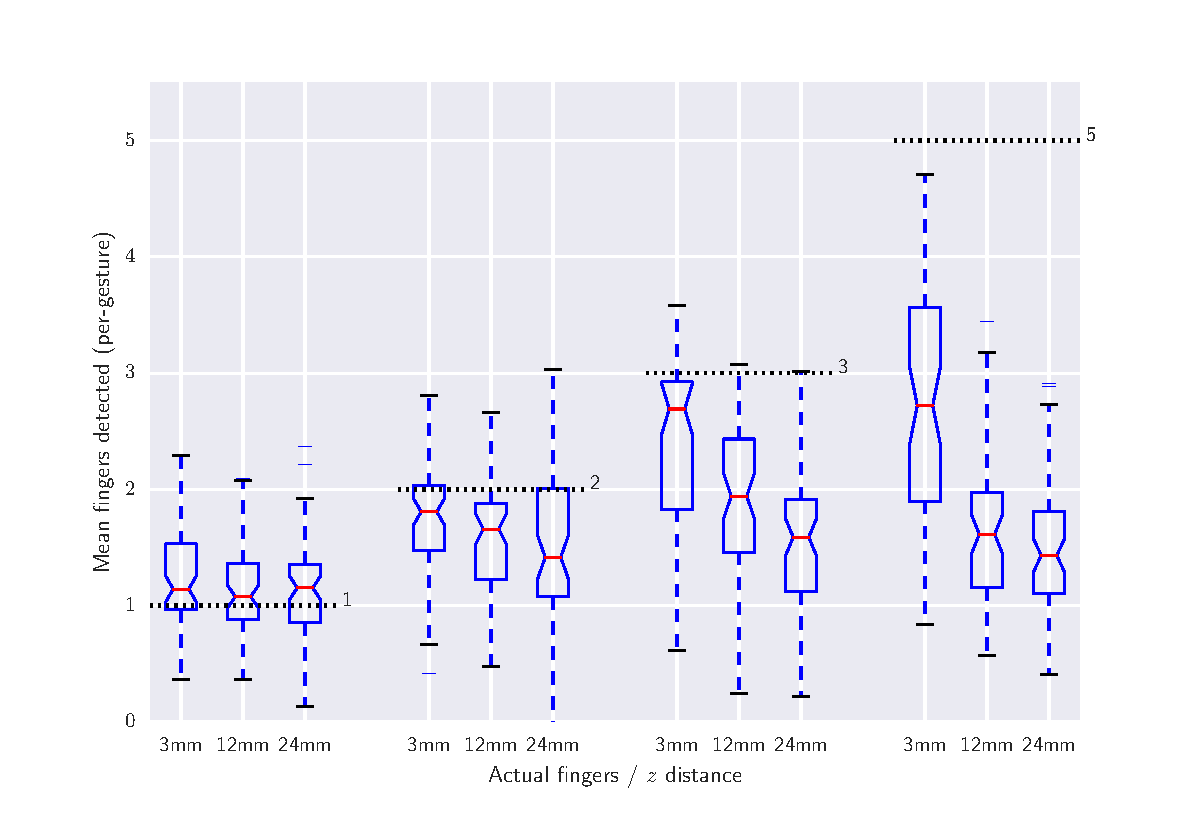
\includegraphics[width=1.0\linewidth]{images/boxplot_finger_distance.pdf}    

    \caption{Average number of fingers detected by the touch sensor at different heights above the surface, averaged over all gestures. Dashed lines indicate
    the true number of fingers present. The Box plots include bootstrapped uncertainty notches for the median. It is clear that the device is biased toward 
    undercounting fingers, particularly at higher $z$ distances.
    }

    % use the notation fig:name to cross reference a figure
    \label{fig:boxplot} 
\end{figure}


%==================================================================================================================================
\chapter{Conclusion}    
Summarise the whole project for a lazy reader who didn't read the rest (e.g. a prize-awarding committee).
\section{Guidance}
\begin{itemize}
    \item
        Summarise briefly and fairly.
    \item
        You should be addressing the general problem you introduced in the
        Introduction.        
    \item
        Include summary of concrete results (``the new compiler ran 2x
        faster'')
    \item
        Indicate what future work could be done, but remember: \textbf{you
        won't get credit for things you haven't done}.
\end{itemize}

%==================================================================================================================================
%
% 
%==================================================================================================================================
%  APPENDICES  

\begin{appendices}

\chapter{Appendices}

Typical inclusions in the appendices are:

\begin{itemize}
\item
  Copies of ethics approvals (required if obtained)
\item
  Copies of questionnaires etc. used to gather data from subjects.
\item
  Extensive tables or figures that are too bulky to fit in the main body of
  the report, particularly ones that are repetitive and summarised in the body.

\item Outline of the source code (e.g. directory structure), or other architecture documentation like class diagrams.

\item User manuals, and any guides to starting/running the software.

\end{itemize}

\textbf{Don't include your source code in the appendices}. It will be
submitted separately.

\begin{table}[!ht]
    \centering
    \rowcolors{2}{}{gray!3}
    \begin{tabular}{@{}l|llllll@{}}
        \textbf{Part} & \textbf{Part Identification} & \textbf{Location} & \textbf{Orientation} & \textbf{Progression}  & \textbf{Error} & \textbf{Other} \\ \hline
        \textbf{1}  & ~ & ~ & ~ & ~ & ~ & ~ \\ 
        \textbf{2}  & ~ & ~ & ~ & ~ & ~ & ~ \\ 
        \textbf{3}  & ~ & ~ & ~ & ~ & ~ & ~ \\ 
        \textbf{4}  & ~ & ~ & ~ & ~ & ~ & ~ \\ 
        \textbf{5}  & ~ & ~ & ~ & ~ & ~ & ~ \\ 
        \textbf{6}  & ~ & ~ & ~ & ~ & ~ & ~ \\ 
        \textbf{7}  & ~ & ~ & ~ & ~ & ~ & ~ \\ 
        \textbf{8}  & ~ & ~ & ~ & ~ & ~ & ~ \\ 
        \textbf{9}  & ~ & ~ & ~ & ~ & ~ & ~ \\ 
        \textbf{10} & ~ & ~ & ~ & ~ & ~ & ~ \\ 
        \textbf{11} & ~ & ~ & ~ & ~ & ~ & ~ \\ 
        \textbf{12} & ~ & ~ & ~ & ~ & ~ & ~ \\ 
        \textbf{13} & ~ & ~ & ~ & ~ & ~ & ~ \\ 
        \textbf{14} & ~ & ~ & ~ & ~ & ~ & ~ \\ 
        \textbf{15} & ~ & ~ & ~ & ~ & ~ & ~ \\ 
        \textbf{16} & ~ & ~ & ~ & ~ & ~ & ~ \\ 
        \textbf{17} & ~ & ~ & ~ & ~ & ~ & ~ \\ 
        \textbf{18} & ~ & ~ & ~ & ~ & ~ & ~ \\ 
        \textbf{19} & ~ & ~ & ~ & ~ & ~ & ~ \\ 
        \textbf{20} & ~ & ~ & ~ & ~ & ~ & ~ \\ 
        \textbf{21} & ~ & ~ & ~ & ~ & ~ & ~ \\ 
        \textbf{22} & ~ & ~ & ~ & ~ & ~ & ~ \\ 
        \textbf{23} & ~ & ~ & ~ & ~ & ~ & ~ \\ 
        \textbf{24} & ~ & ~ & ~ & ~ & ~ & ~ \\ 
        \textbf{25} & ~ & ~ & ~ & ~ & ~ & ~ \\ 
        \textbf{26} & ~ & ~ & ~ & ~ & ~ & ~ \\ 
        \textbf{27} & ~ & ~ & ~ & ~ & ~ & ~ \\ 
        \textbf{28} & ~ & ~ & ~ & ~ & ~ & ~ \\ 
        \textbf{29} & ~ & ~ & ~ & ~ & ~ & ~ \\ 
        \textbf{30} & ~ & ~ & ~ & ~ & ~ & ~ \\ 
        \textbf{31} & ~ & ~ & ~ & ~ & ~ & ~ \\ 
        \textbf{32} & ~ & ~ & ~ & ~ & ~ & ~ \\ 
        \textbf{33} & ~ & ~ & ~ & ~ & ~ & ~ \\ 
        \textbf{34} & ~ & ~ & ~ & ~ & ~ & ~ \\ 
        \textbf{35} & ~ & ~ & ~ & ~ & ~ & ~ \\ 
        \textbf{36} & ~ & ~ & ~ & ~ & ~ & ~ \\ 
        \textbf{37} & ~ & ~ & ~ & ~ & ~ & ~ \\ 
        \textbf{38} & ~ & ~ & ~ & ~ & ~ & ~ \\ 
        \textbf{39} & ~ & ~ & ~ & ~ & ~ & ~ \\ 
        \textbf{40} & ~ & ~ & ~ & ~ & ~ & ~ \\ 
        \textbf{41} & ~ & ~ & ~ & ~ & ~ & ~ \\ 
        \textbf{42} & ~ & ~ & ~ & ~ & ~ & ~ \\ 
        \textbf{43} & ~ & ~ & ~ & ~ & ~ & ~ \\ 
        \textbf{44} & ~ & ~ & ~ & ~ & ~ & ~ \\ 
        \textbf{45} & ~ & ~ & ~ & ~ & ~ & ~ \\ 
        \textbf{46} & ~ & ~ & ~ & ~ & ~ & ~ \\ 
        \textbf{47} & ~ & ~ & ~ & ~ & ~ & ~ \\ 
        \textbf{48} & ~ & ~ & ~ & ~ & ~ & ~ \\ 
        \textbf{49} & ~ & ~ & ~ & ~ & ~ & ~ \\ 
        \textbf{50} & ~ & ~ & ~ & ~ & ~ & ~ \\ 
        \textbf{51} & ~ & ~ & ~ & ~ & ~ & ~ \\ 
        \textbf{52} & ~ & ~ & ~ & ~ & ~ & ~ \\ 
        \textbf{53} & ~ & ~ & ~ & ~ & ~ & ~ \\ 
        \textbf{54} & ~ & ~ & ~ & ~ & ~ & ~ \\ 
        \textbf{55} & ~ & ~ & ~ & ~ & ~ & ~ \\ 
        \textbf{56} & ~ & ~ & ~ & ~ & ~ & ~ \\ 
        \textbf{57} & ~ & ~ & ~ & ~ & ~ & ~ \\ 
        \textbf{58} & ~ & ~ & ~ & ~ & ~ & ~ \\ 
        \textbf{59} & ~ & ~ & ~ & ~ & ~ & ~ \\ 
    \end{tabular}
\end{table}

\end{appendices}

%==================================================================================================================================
%   BIBLIOGRAPHY   

% The bibliography style is abbrvnat
% The bibliography always appears last, after the appendices.

\bibliographystyle{abbrvnat}

\bibliography{l4proj}

\end{document}
